\documentclass{article}
\usepackage{graphicx}
\usepackage{float}
\usepackage{amsmath}
\graphicspath{{images/}}
\usepackage{caption}
\captionsetup[figure]{position = below,}
\usepackage{listings}
\usepackage{xcolor}
\usepackage{amssymb}
 \usepackage{amsthm}
 \usepackage{amsfonts}
\usepackage{braket}
\DeclareCaptionFont{white}{\color{white}}
\DeclareCaptionFormat{listing}{%
\parbox{\textwidth}{\colorbox{gray}{\parbox{\textwidth}{#1#2#3}}\vskip-4pt}}
\captionsetup[lstlisting]{format=listing,labelfont=white,textfont=white}
\lstset{frame=lrb,xleftmargin=\fboxsep,xrightmargin=-\fboxsep, columns=fullflexible}


\title{\textbf{Super dense coding protocol in Python}}

\author{Indranil Ghosh\\Jadavpur University, Physics Department\\Email: indranilg49@gmail.com}

\date{\today}

\begin{document}
\maketitle

\begin{abstract}
This Project is to simulate the  Superdense Coding, a simple application of elimentary Quantum mechanics and computations. A Python program has been designed, available in Github (https://github.com/indrag49/Quantum-SimuPy) , to accompany this project. Packages used: Numpy, Pandas and Mathplotlib. The quantum gates and the functions required for this simulation are available in the program and can be easily implemented. The moto of this project is to use python packages to design a quantum simulator for performing simple quantum computations.
\end{abstract}

\section{Introduction}
Super Dense Coding protocol was first introduced by Bennet and Wiesner in 1992. In this protocol a number of classical bits is shared between two parties by sharing a few qubits. It consists of two parts: 1) A set of instructions and 2) the deseired results. The protocol is considered to be correct if and only if the set of instructions leads to the desired results. Quantum Entanglement, also described by Einstein as "Spooky action at a distance" is the key resource in Super Dense Coding.  \\ \par
This protocol involves two parties \textit{Alice} and \textit{Bob} who are located at a long distance from one another. Alice has in possession two classical bits of information which she tends to share with  Bob by sending only a single qubit to Bob.

\section{Procedure}
\begin{figure}[H]
\centering 
\noindent\makebox[\textwidth]{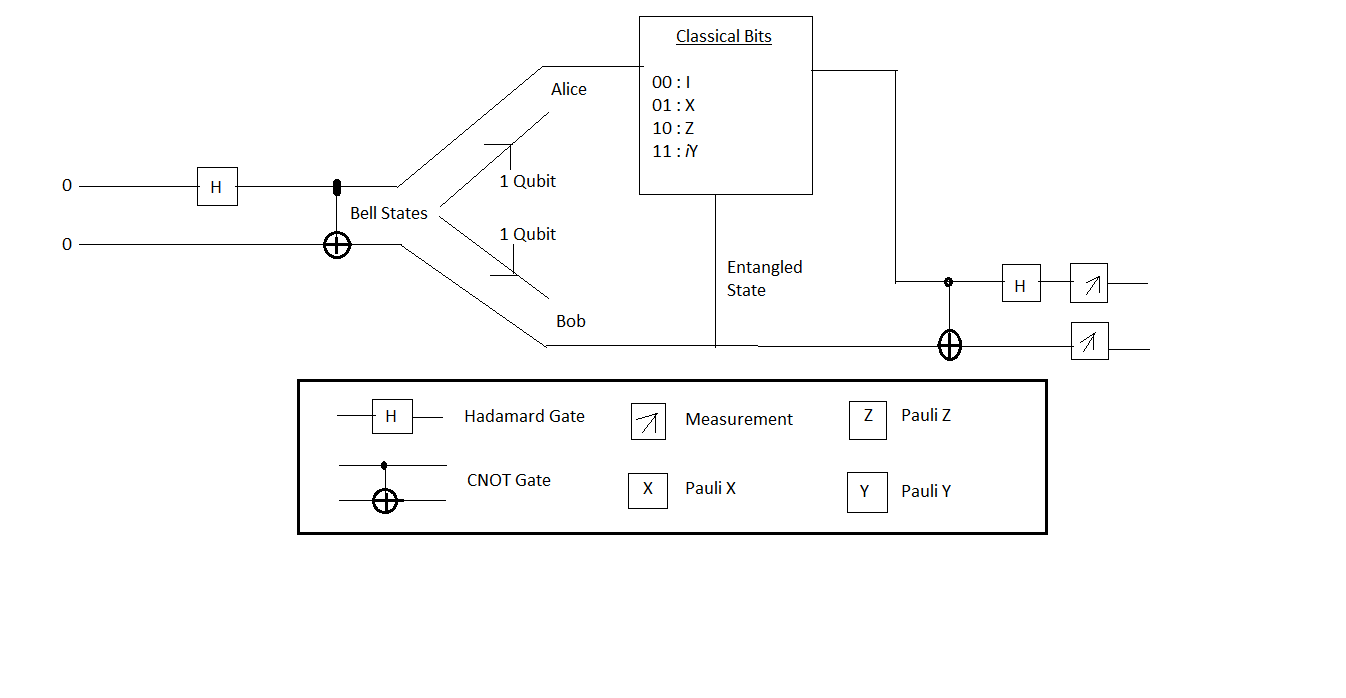
\includegraphics[scale=0.4]{SuperDense}}%
\caption{SuperDense Coding Protocol}
\end{figure}
At first, we prepare the entangled Bell states. We apply $H \otimes I$ unitary operation on the input qubits followed by the CNOT unitary operation(control=0 , target=1). The output we get is the entangled Bell state. We can have 4 Bell states corresponding to inputes: $\ket{00}$, $\ket{01}$, $\ket{10}$ and $\ket{11}$ \\ \par
\begin{center}
\begin{tabular}{||c c ||}
\hline
Input & Output \\ [0.5ex]
\hline
\hline
$\ket{00}$ & $(\ket{00}+\ket{11}) \over \sqrt{2}$ \\
\hline
\hline
$\ket{01}$ & $(\ket{01}+\ket{10}) \over \sqrt{2}$ \\
\hline
\hline
$\ket{10}$ & $(\ket{00}-\ket{11}) \over \sqrt{2}$ \\
\hline
\hline
$\ket{11}$ & $(\ket{01}-\ket{10}) \over \sqrt{2}$ \\
\hline
\end{tabular}
\end{center}

While computing the Bell states we should remember that to calculate the equivalent gate matrix of two parallel gate matrices, we should compute their tensor product. Using my Python program,\\ \par
\begin{lstlisting}[language=Python, frame=single]
def B(Qubit):
        H=Hadamard(I2)
        b=CNOT(np.kron(H, I2))
        return b.dot(Qubit)
b00=B(Q00)
b01=B(Q01)
b10=B(Q10)
b11=B(Q11)
\end{lstlisting} 
The bell states \textit{b00}, \textit{b01}, \textit{b10} and \textit{b11} are prepared. In the Super dense coding protocol we use the Bell state $(\ket{00}+\ket{11}) \over \sqrt{2}$, i.e., we input $\ket{00}$  to prepare , as shown in Figure 1. Alice and Bob share this pair of qubits in the entangled state, initially. Alice possesses the first qubit, while Bob, the second. By sending the single qubit in her possession, Alice can easily transfer two bits of classical information to Bob.\\ \par
Now, Alice follows the following rule: \\  \par
\begin{figure}[H]
\centering 
\noindent\makebox[\textwidth]{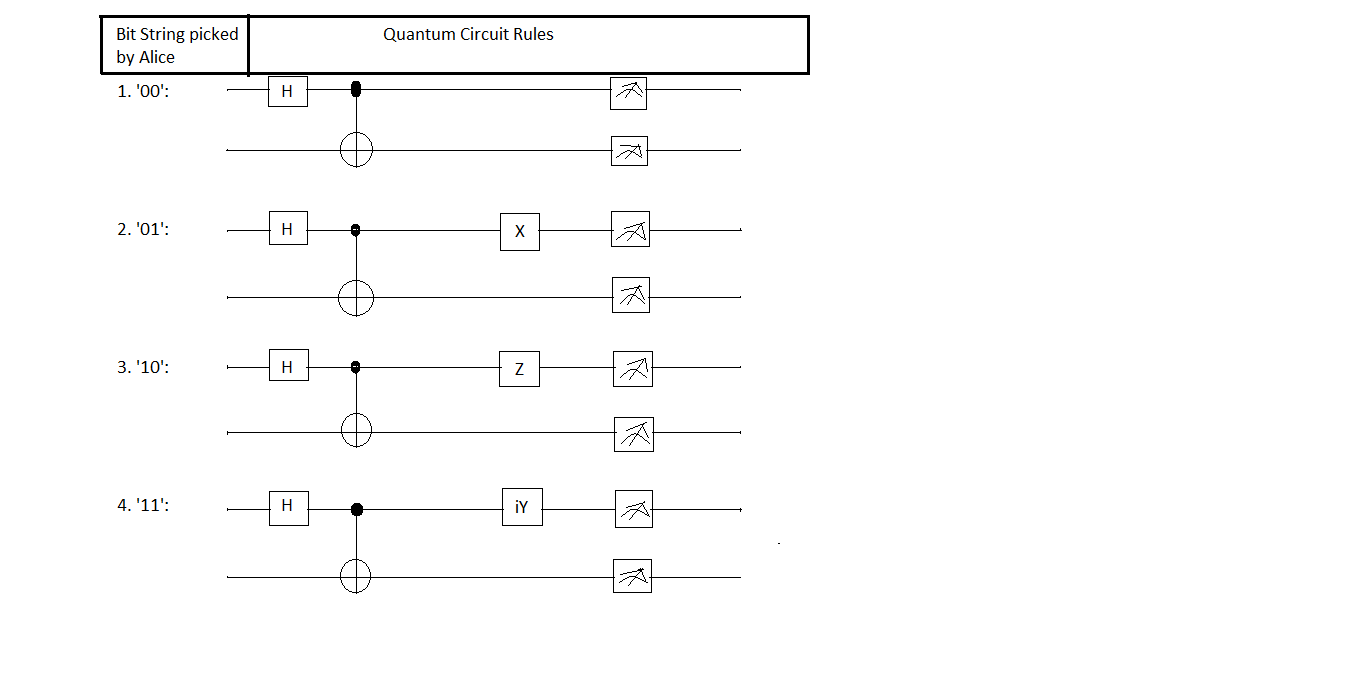
\includegraphics[scale=0.4]{superdense2}}%
\caption{Rules followed by Alice}
\end{figure}

Input: $(\ket{00}+\ket{11}) \over \sqrt{2}$\\ \par
Output:\\ \par
\begin{center}
\begin{tabular}{||c c c||}
\hline
Bit String picked by Alice & Gate Applied & Output\\[0.5ex]
\hline
\hline
'00' & I & $(\ket{00}+\ket{11}) \over \sqrt{2}$ \\
\hline
\hline
'01' & X & $(\ket{10}+\ket{01}) \over \sqrt{2}$ \\
\hline
\hline
'10' & Z & $(\ket{00}-\ket{11}) \over \sqrt{2}$ \\
\hline
\hline
'11' & iY & $(\ket{01}-\ket{10}) \over \sqrt{2}$ \\
\hline
\end{tabular}
\end{center}

\begin{lstlisting}[language=Python, frame=single]
def Alice(Q):
        if Q=="00": L=np.kron(I2, I2)
        elif Q=="10":
                z=PauliZ(I2)
                L=np.kron(z, I2)
        elif Q=="01":
                x=PauliX(I2)
                L=np.kron(x, I2)
        else:
                y=PauliY(I2)
                L=np.kron(1j*y, I2)
        return L.dot(b00)
\end{lstlisting} 
The four resulting states are again the Bell states/ \textit{EPR} pairs. They are mutually orthonormal to one another and can be determined by appropriate quantum measurement. To check whether two of the Bell states are orthonormal we calculate their inner product  and obtain the result 0. We check some of these examples, using python program:\\ \par

\begin{lstlisting}[language=Python, frame=single]
>>> np.inner(b00, b01)
0.0
>>> np.inner(b01, b10)
0.0
>>> np.inner(b00, b10)
0.0
>>> np.inner(b01, b11)
0.0
\end{lstlisting} 

Now, Bob already has a qubit and after receiving the qubit from Alice, he does a measurement in the Bell basis and extracts the result, i.e., determines which of the four classical bit strings Alice sent him. Bob at first  applies the CNOT unitary operation followed by $H \otimes I$ unitary operations, on the \textit{EPR} pairs i.e, the reverse of the operations used while preparing the Bell states, to obtain the origibnial classiical bits sent by Alice.\\ \par
\begin{center}
\begin{tabular}{||c c||}
\hline
Bell States & Output\\[0.5ex]
\hline
\hline
$\ket{b00}$ & $\ket{00}$ \\
\hline
\hline
$\ket{b01}$ & $\ket{01}$ \\
\hline
\hline
$\ket{b10}$ & $\ket{10}$ \\
\hline
\hline
$\ket{b11}$ & $\ket{11}$ \\
\hline
\end{tabular}
\end{center}
 \begin{lstlisting}[language=Python, frame=single]
def Bob(Qubit):
        s=CNOT(Qubit)
        return s.dot(np.kron(Hadamard(I2), I2))
\end{lstlisting} 

If a hacker, Ada, intercepts Alice's qubit en route to Bob, all she obtains is a part of the entangled state and no useful information is stolen by her, untill and unless she interacts with Bob's qubit.
\begin{thebibliography}{9}
\bibitem{knuthwebsite}
\texttt{http://www-reynal.ensea.fr/docs/iq/QC10th.pdf}
\bibitem{knuthwebsite}
\texttt{https://github.com/indrag49/Quantum-SimuPy}
\end{thebibliography}
\end{document}
